\documentclass{report}
\usepackage[utf8]{inputenc}
\usepackage{graphicx}
\usepackage{hyperref}

\title{Emotion Creators: The Sensible Manual}
\author{Kasanari}

\begin{document}


\begin{titlepage}
\maketitle
\end{titlepage}




\begin{titlepage}
\begin{center}
    This document is dedicated to all the hard working people making mods and translations for Illusion's unique, but often slightly broken games.
\end{center}
\end{titlepage}



\newpage

\pagenumbering{arabic}
\setcounter{page}{1}

\chapter{Technical Stuff}

Install the Hongfire Patch by Marco.

\chapter{Introduction}

\section{What is Emotion Creators?}

\textit{Emotion Creators} is a tool/game for making and viewing visual novels. It is made by the Japanese game company \textit{Illusion}. EC shares a lot of its DNA with Illusion's previous title \textit{Koikatsu}. This manual assumes you are at least somewhat familiar with Koikatsu.

\section{Character Maker}

The character maker works in a similar way to the one in Koikatsu, if you have played Koikatsu you know what to expect. There are some differences however.
\begin{itemize}
    \item Characters can only store one outfit.
    \item There is a jazzy song playing in the background.
\end{itemize}

Worth noting is that the personality you choose for you character determines their voice in-game. This can not be changed in other parts so make sure to pick the right settings now.

\section{Map Maker}

The map maker is where you create maps.

\section{Pose Maker}

The scene maker exists to create preset poses that can be used within you visual novels. You can set up poses using IK or FK, with existing poses as basis. The pose maker is also accessible from the \textit{ADV Scene Maker}.

\chapter{The Scene Maker}

\section{Setting Up}

Before starting on your Mongolian slideshow you have to setup some things. After selecting the option to make a new scene you will be prompted by a screen like the one in \autoref{fig:scene_startup}. Most settings can be changed later, with one important exception.
\textbf{You can not change the number of characters after this step. You can not change the gender of existing characters either.} As such, if you are unsure of what characters may appear in your story it may be good to add a couple of male and female characters just to be safe. After adding some characters, you will be sent to the \textit{Node Chart}.

\begin{figure}[!htpb]
    \centering
    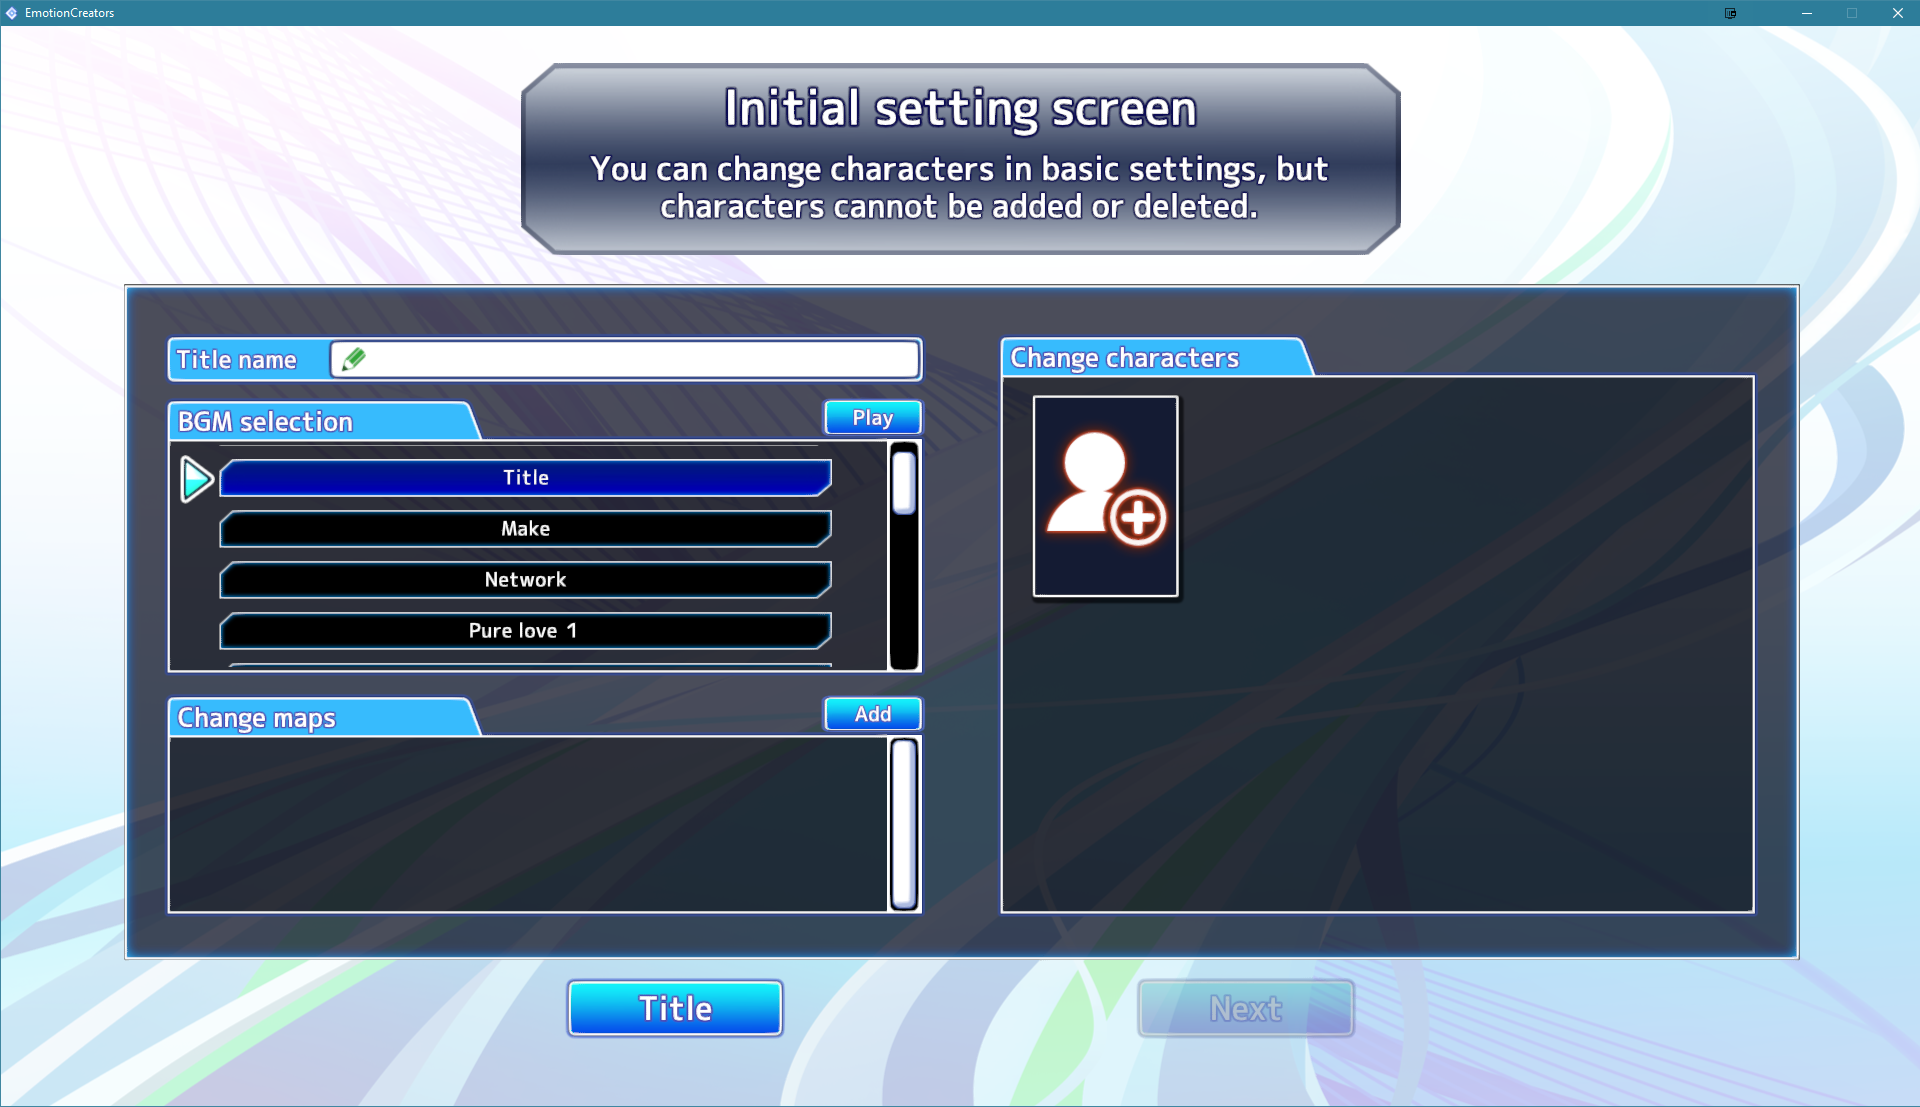
\includegraphics[width=\textwidth]{Figures/scene_startup.PNG}
    \caption{The screen for setting up new scene.}
    \label{fig:scene_startup}
\end{figure}

By pressing \textit{Basic Settings} from this screen you will go back to the screen we first saw when making the scene. From here you can pick the default music, change the name of your game, change characters and add more maps. This is also where you will save your game, if you consider the smut you made worth saving.

\section{The Node Chart}

The \textit{Node Chart} is the screen from which you manage the flow of you story. In other words, where the story will start, where it will end and what scenes will lead to one another. There are two types of scenes which can be added to your story, \textit{ADV Nodes} and \textit{H Nodes}. The \texttt{Check Data} button will verify that your game is playable, which mainly means that there exists a path from beginning to end and that there are no dead ends. \texttt{Test play} lets you play through your game from the beginning, note that you can not test your game unless it is verified as working by the same metrics as \texttt{Check Data}.

\begin{figure}[!htpb]
    \centering
    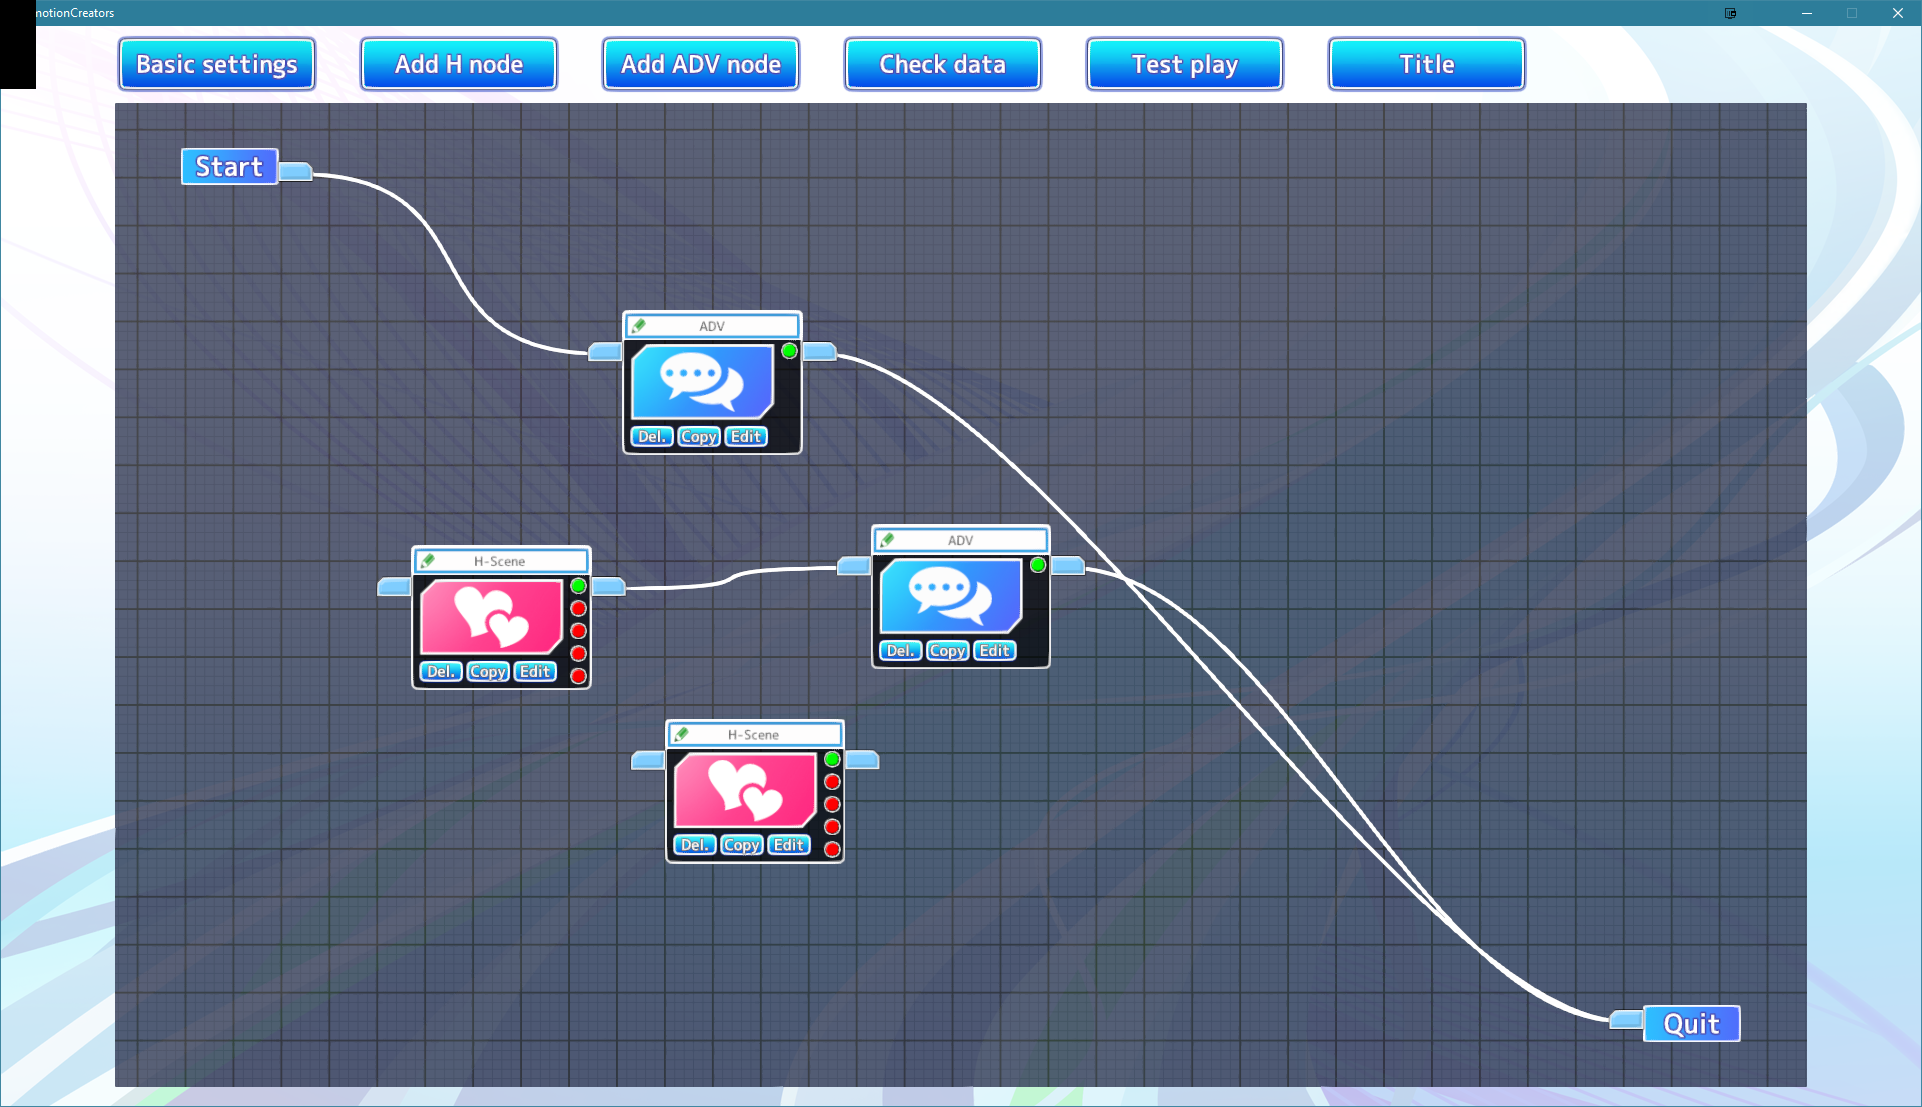
\includegraphics[width=\textwidth]{Figures/noide_chart.PNG}
    \caption{The node chart.}
    \label{fig:node_chart}
\end{figure}

Nodes have green spheres on the right edges representing multiple endings in the scenes. ADV Node initially only have one exit, but more can be added within the \textit{ADV Scene Maker}.

\begin{figure}[!htpb]
    \centering
    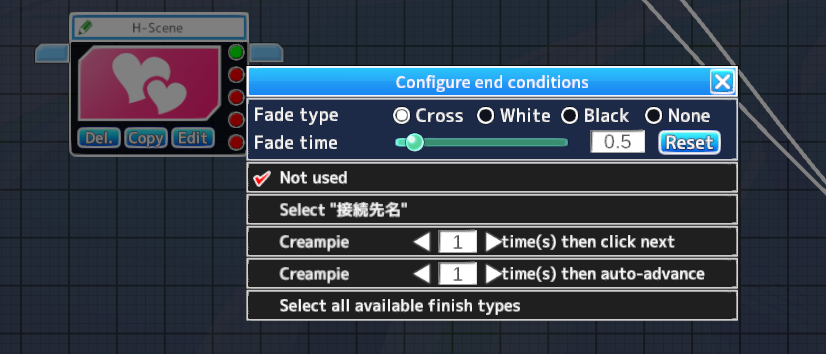
\includegraphics[width=\textwidth]{Figures/h_node.PNG}
    \caption{Scene transition conditions for H Node.}
    \label{fig:hnode}
\end{figure}

\section{The ADV Scene Maker}

\textit{ADV Nodes} are where the visual novel sections of the game happen. This is the type of gameplay you would traditionally associate with the genre.

The 

\section{The H Scene Maker}

\textit{H Nodes} allow you to make semi-interactive sex scenes for your adventure. Sex scenes will usually play out in the following way:

\begin{enumerate}
    \item Wait for sex.
    \item Have sex.
    \item Cum.
    \item Repeat from step 2. or keep going with the story.
\end{enumerate}

Some parts of this process can be modified, as explained later but this shows the general flow.

When first entering the maker you will be prompted with the screen shown in \ref{fig:hscenestart}. From here you can pick which parts of the human mating procedure you wish to include. \texttt{Idle} is the first scene which is loaded when entering the H Scene, this is usually where the characters are waiting for the process to begin. The \texttt{Idle} scene is only entered once and will lead into the \texttt{Loop} scene.

The \texttt{Loop} scene is the main part of the H scene. This is where docking procedure, knob polishing or fucking takes place. The \texttt{Loop} scene 

\begin{figure}[!htpb]
    \centering
    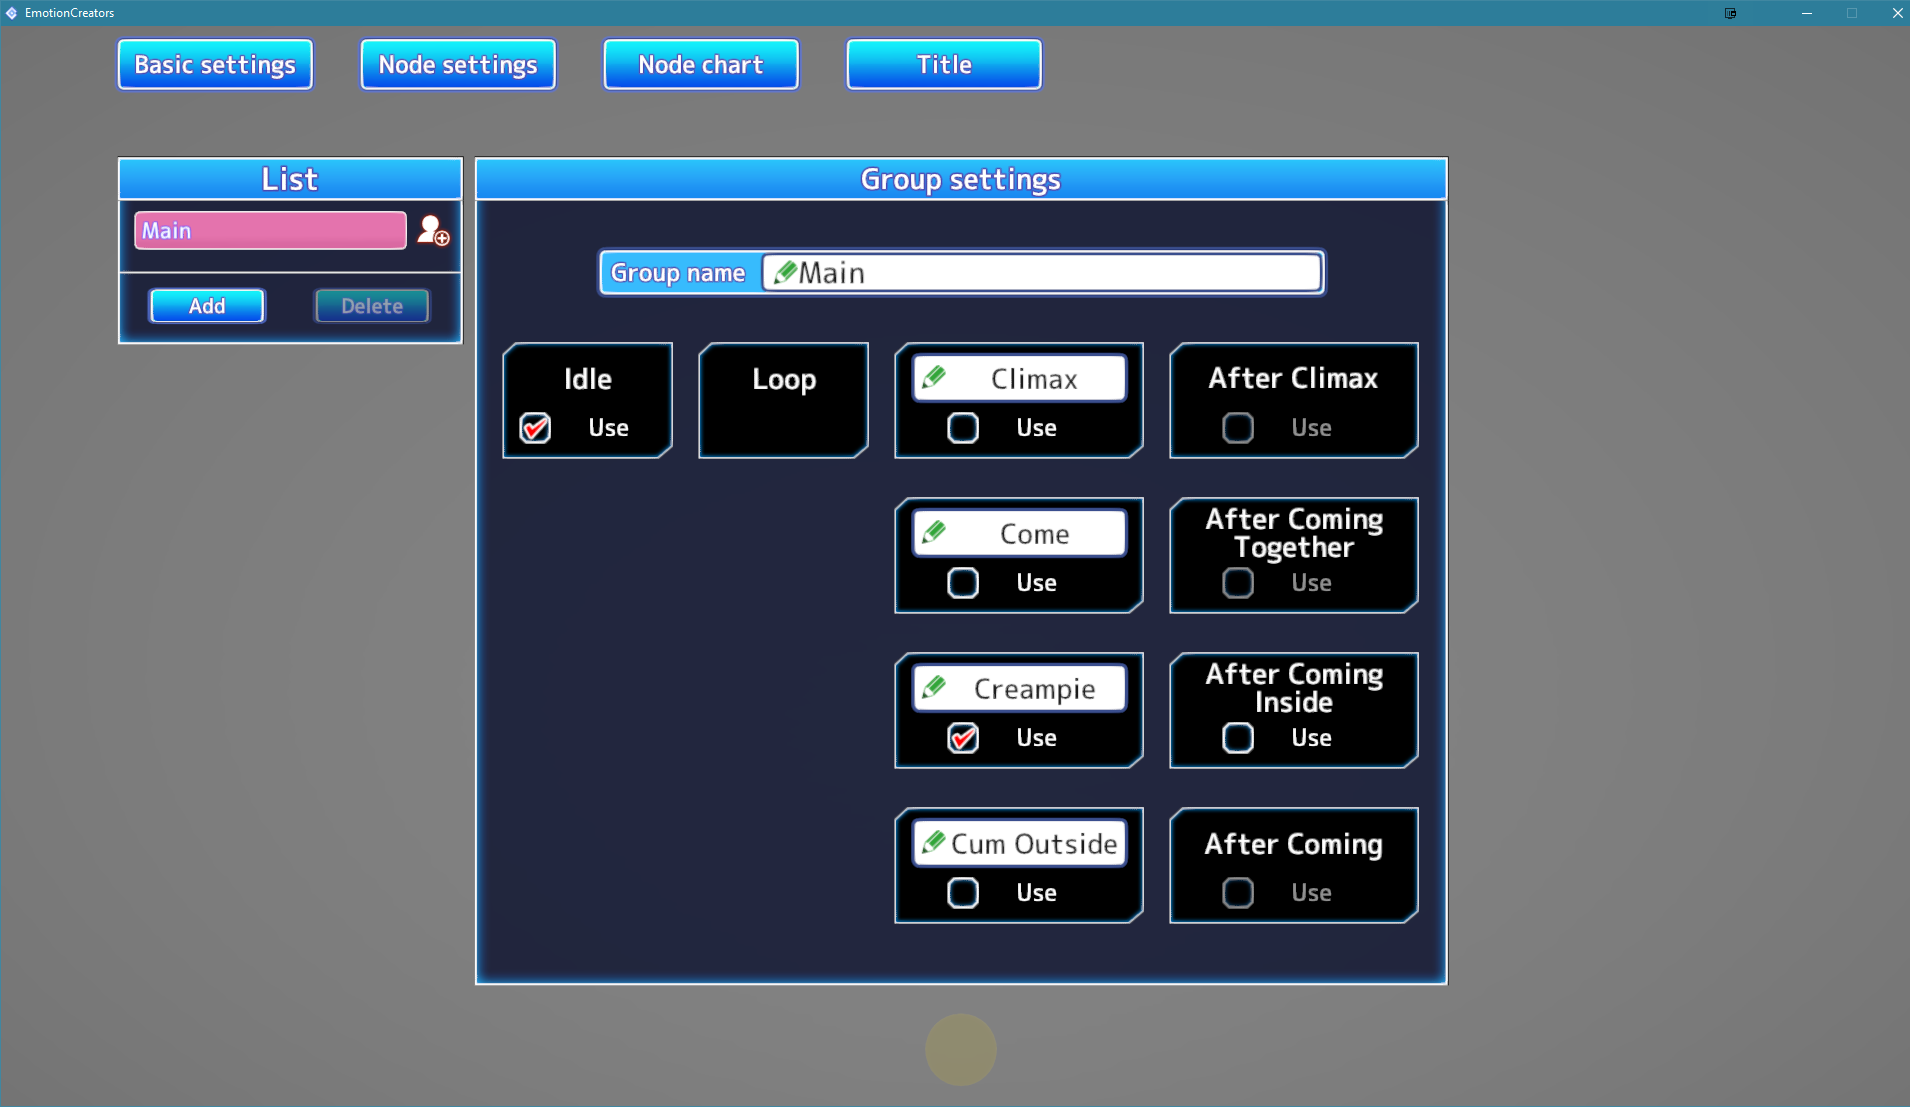
\includegraphics[width=\textwidth]{Figures/hscenestartup.PNG}
    \caption{Scene transition conditions for H Node.}
    \label{fig:hscenestart}
\end{figure}

\subsection{}


\end{document}
